\documentclass[12pt,a4paper]{article}

\usepackage{t1enc}
\usepackage[utf8]{inputenc}
\usepackage[magyar]{babel}
% KP kihuztam a makeidx es natbib csomagot, nalam hibat jelzett
%\usepackage{makeidx} 
%\usepackage{natbib}
\usepackage{enumitem}
\usepackage[version=4]{mhchem}
\usepackage{graphicx}
\usepackage{tabu}
\usepackage{makecell}
\usepackage{enumitem}

\usepackage{amsmath}
\usepackage{amssymb}
\usepackage{amsthm}

\usepackage{tikz}
\usetikzlibrary{positioning}

\author{Gáspár Tamás}
\title{A PageRank és kiszámolása}
\date{}

% számláló és formázás definícióknak: \begin{definicio}
\newcounter{definicioszam}
\newenvironment{definicio}[1]
{{\medskip}\noindent \stepcounter{definicioszam}
%{\bfseries{\thedefinicioszam. Definíció: #1\\[1ex]}}}{\bigskip }
{\bfseries{\thedefinicioszam. Definíció: \textit{#1.}}}}{\bigskip }
% szerintem igy jobb a definicio kornyezet KP

% a vektorokat jelolheted felkoverrel, hogy megkonnyitsd a megertest: KP
\newcommand{\bx}{\mathbf{x}}
\newcommand{\be}{\mathbf{e}}
\newcommand{\by}{\mathbf{y}}

\newtheorem{tetel}{Tétel}
\newtheorem{lemma}{Lemma}[tetel]

\begin{document}

%FŐOLDAL ------------------------------------------------------------------

%intézet
\thispagestyle{empty}
\centerline{\textsc{\Large{Szegedi Tudományegyetem}}}
\vspace{0.3 cm}
\centerline{\textsc{\Large{Természettudományi és Informatikai Kar}}}

\vspace*{2 cm}

\centerline{\textsc{\Large{Bolyai Intézet}}}
\vspace{0.3 cm}
\centerline{\textsc{\Large{Sztochasztika tanszék}}}

\vspace{3 cm}

%cím
\centerline{\LARGE{A PageRank és kiszámolása}}
\vspace{0.5 cm}
\centerline{\Large{\textsc{Szakdolgozat}}}

\vspace{3 cm}

%készítő és témavezető táblázat
\begin{center}
	\begin{tabu} to \textwidth { X[l]  X[r] }
		\makecell[l]{Készítette: Gáspár Tamás \\ Matematika BSc hallgató} &
		 \makecell[r]{Témavezető: Dr. Kevei Péter \\ Egyetemi docens \\ Sztochasztika tanszék} \\
	\end{tabu}
\end{center}

\vspace{3 cm}

\centerline{\Large{\textsc{Szeged, 2019}}}

%tartalomjegyzék oldala -------------------------------------------------
\newpage
\thispagestyle{empty}

\tableofcontents

%tényleges kezdet --------------------------------------------------------
\newpage
\setcounter{page}{1}
\fontsize{12}{16}\selectfont

\section{Bevezető}

Dolgozatom témája a PageRank, és az ennek számolásához használt algoritmus, melynek legfőbb alkalmazási területe az internetes weboldalak bizonyos szempontok szerinti rangsorolása.

Ez a fejezet röviden ismerteti a PageRank történetét és megemlít egy, a PageRank számolásához használható, általam készített programot. A következő fejezet a PageRank tárgyalásához szükséges alapvető fogalmakat és definíciókat vezet be. 

\subsection{A PageRank algoritmus története}

A PageRank algoritmust Larry Page és Sergei Brin alkották meg 1998-ban, a Standford Egyetem hallgatóiként. Arra kerestek megoldást, hogy miként lehet az akkoriban robbanásszerű növekedésnek induló internet weboldalait rangsorolni, mivel látszott, hogy az akkor alkalmazott keresőmotorok erre már hamarosan nem lesznek képesek.

Úgy gondolták, hogy a rangsorolás alapja az internet hiperlink struktúrája kell hogy legyen. Feltették, hogy ha egy oldal linkel egy másikra, az kifejezi azt, hogy az oldal készítői megbíznak a linkelt oldalban, ezért az algoritmusukat úgy építették fel, hogy egy oldal fontossága (ezt szintén PageRanknak nevezik) attól függ, hogy mennyi és milyen fontos oldalak linkelnek rá.

Larry Page és Sergei Brin találmánya olyan jól alkalmazhatónak bizonyult, hogy Google néven saját vállalkozást alapítottak. A cég keresőmotorjának alapja máig a PageRank algoritmus, skálázhatóságát mutatja, hogy a Google ma már több mint 130 billió weboldalt indexel. 

\subsection{PageRank program}\label{program}

Dolgozatomhoz grafikus felhasználói felülettel ellátott asztali alkalmazást is készítettem, Java nyelven. Ez a program képes előre megadott oldalszámú webet különböző paraméterek alapján véletlenszerűen generálni, majd ehhez PageRankot számolni. A 150 oldalnál kisebb méretű webekhez tartozó mátrixokat meg is tudja jeleníteni.

A program és annak forráskódja is letölthető a következő oldalról:

\vspace{0.3 cm}
\textit{https://github.com/Gtomika/PageRank/releases/tag/v4.1}
\vspace{0.3 cm}

 A futtatáshoz a számítógépen telepítve kell hogy legyen a Java 8-as, vagy újabb verziója.

\section{Alapfogalmak és definíciók}

\subsection{Linkek, web és a lógó oldalak}\label{link_web_logooldal}

Ahhoz hogy PageRankról beszélhessünk, először a web fogalmát kell bevezetni.

\begin{definicio}{Linkhalmaz}
	Legyen V a weboldalak halmaza. Ekkor $L \subset V \times V$ \textbf{linkhalmaz}ban $(v_1, v_2) \in V$ pontosan akkor van benne ha $v_1$ oldalon van $v_2$-re mutató link. 
\end{definicio}

\begin{definicio}{Web}
	Legyen $V$ a weboldalak halmaza, $L$ pedig az ehhez tartozó linkhalmaz. Ekkor a web egy irányított gráf, melynek csúcsai $V$ elemei, élei pedig $L$ elemei, ahol ha $v_1, v_2 \in V$ és $(v_1,v_2) \in L$, akkor az él $v_1$-ből $v_2$-be mutat. 
\end{definicio}

\begin{figure}[h]
	\centering
	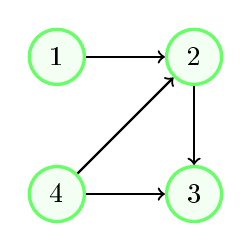
\begin{tikzpicture}[
	roundnode/.style={circle, draw=green!60, fill=green!5, very thick, minimum size=7mm},
	]
	\centering
	%Nodes
	\node[roundnode]      (c1)                     {1};
	\node[roundnode]      (c2)       [right=of c1] {2};
	\node[roundnode]      (c3)       [below=of c2] {3};
	\node[roundnode]      (c4)       [below=of c1] {4};
	
	%Lines
	\draw[->,thick] (c1) -- (c2);
	\draw[->,thick] (c2) -- (c3);
	\draw[->,thick] (c4) -- (c2);
	\draw[->,thick] (c4) -- (c3);
	\end{tikzpicture}
	\caption{Egy 4 oldalból álló web}
\end{figure}

A linkhalmaz definíciója ugyan megengedi azt, hogy egy oldal önmagára linkeljen, mert bár egy valós web esetén ez lehetséges, de a PageRank algoritmus esetén nem akarjuk, hogy az ilyen linkek is beleszámítsanak a rangsorolásba. Ezeket a linkeket ezért egyszerűen elhagyjuk.

Az is megfigyelhető, hogy a definíciókban a linkeknek nincsen multiplicitása, egy oldal vagy linkel egy másikra, vagy nem. Ez azért van, hogy a rangsorolást ne lehessen olyan egyszerűen manipulálni, hogy bizonyos oldalak sok linket tartalmaznak egy másikra.  

Előfordulhat olyan web, ahol bizonyos oldalakról nincsenek kimenő linkek. Az ilyen oldalakat lógó oldalnak nevezzük (azokat a linkeket amelyek rájuk mutatnak pedig lógó linkeknek). A későbbiekben ezek az oldalak problémákat okoznak, ezért megadunk egy módszert, mellyel a ezeket az oldalakat el lehet tüntetni: minden lógó oldalt helyettesítünk egy, az összes másik oldalra linkelővel (ebben a kivételes esetben megengedjük az önmagára linkelést is). 

\bigskip

\begin{minipage}{0.4\textwidth}
	\begin{center}
		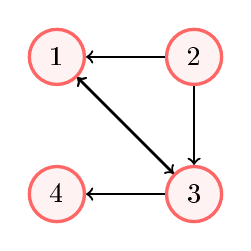
\begin{tikzpicture}[
		roundnode/.style={circle, draw=red!60, fill=red!5, very thick, minimum size=7mm},
		]
		%Nodes
		\node[roundnode]      (c1)                     {1};
		\node[roundnode]      (c2)       [right=of c1] {2};
		\node[roundnode]      (c3)       [below=of c2] {3};
		\node[roundnode]      (c4)       [below=of c1] {4};
		
		%Lines
		\draw[->,thick] (c1) -- (c3);
		\draw[->,thick] (c2) -- (c3);
		\draw[->,thick] (c3) -- (c1);
		\draw[->,thick] (c3) -- (c1);
		\draw[->,thick] (c3) -- (c4);
		\draw[->,thick] (c2) -- (c1);
		\end{tikzpicture}
	\end{center}
\end{minipage}
\begin{minipage}{0.5\textwidth}
	\begin{center}
		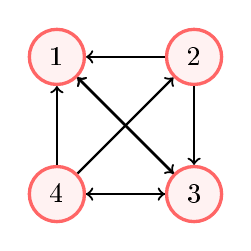
\begin{tikzpicture}[
	roundnode/.style={circle, draw=red!60, fill=red!5, very thick, minimum size=7mm},
	]
	%Nodes
	\node[roundnode]      (c1)                     {1};
	\node[roundnode]      (c2)       [right=of c1] {2};
	\node[roundnode]      (c3)       [below=of c2] {3};
	\node[roundnode]      (c4)       [below=of c1] {4};
	
	%Lines
	\draw[->,thick] (c1) -- (c3);
	\draw[->,thick] (c2) -- (c3);
	\draw[->,thick] (c3) -- (c1);
	\draw[->,thick] (c3) -- (c1);
	\draw[->,thick] (c3) -- (c4);
	\draw[->,thick] (c2) -- (c1);
	\draw[->,thick] (c4) -- (c1);
	\draw[->,thick] (c4) -- (c2);
	\draw[->,thick] (c4) -- (c3);
	\end{tikzpicture}
	\end{center}
\end{minipage}

\bigskip
\centerline{Egy lógó oldallal (4) rendelkező web, és ugyanez a web, helyettesített oldallal.}

\vspace{0.5 cm}

A helyettesítés mögötti heurisztika az, hogy ha egy böngésző egy olyan oldalra érkezik, ahonnan a linkeken keresztül nem tud továbbmenni, akkor véletlenszerűen, egyenletes eloszlás szerint választ az összes oldal közül.

\subsection{A PageRank definíciója}

Egy oldal fontossága azon múlik, hogy mennyi oldal linkel rá, és hogy ezek milyen fontosak. A linkelő oldalak fontosságára azért van szükség, mert enélkül egy oldaltulajdonos tudná úgy növelni a weboldalának fontosságát, hogy rengeteg oldalt hoz létre, melyek mind linkelnek egymásra és a saját oldalára (ezt link farmnak nevezik \cite{lang}).

Egy webet el lehet úgy is képzelni, mint az oldalak demokráciáját ahol minden oldalnak egy szavazata van és ezt a szavazatot (és még a kapott szavazatokat is) továbbosztja úgy, hogy linkel a többi oldalra.

\begin{definicio}{Weboldal PageRankja}
	Legyen adott egy web, $V$ az oldalak, $L$ a linkek halmaza.
	Legyen $v_i \in V$ oldal PageRankja $r(v_i)$, az oldalról kimenő linkek száma pedig $ |v_i| $. 
	
	Jelölje $B_i \subset V$ azon oldalak halmazát amelyen linkelnek $v_i$-re, azaz
	\[B_i = \{ v_j \in V: \exists l \in L, \quad l = (v_j,v_i) \} \text{.} \]
	Ekkor $v_i$ oldal PageRank-ja definíció szerint:
	
	\[ r(v_i) = \sum_{v_j \in B_i} \frac{r(v_j)}{ |v_j| } \text{.} \]
\end{definicio}

A definícióban megjelenik az is, hogy egy oldalnak mennyi kimenő linkje van. Minél több oldalra linkel, annál kevesebbet fog számítani az ő linkjének értéke. Ez ellensúlyozza a már említett link farmokat.

A szummában szereplő oldalak egyikénél sem lehet a kimenő linkek száma nulla, mert mindegyik oldal eleme a $B_i$ halmaznak, azaz legalább $v_i$-re linkelnek. Előfordulhat, hogy egy oldalra nincs egyetlen link sem. A definícióban ilyenkor egy üres összeg szerepel, azaz az oldal rangja 0.

A PageRank definíciója tehát rekurzív. Egy oldal rangjának meghatározásához minden rá linkelő oldal rangját ismernünk kell. Ha a webünk $n$ db oldalt tartalmaz, akkor a definíció meghatároz $n$ db lineáris egyenletet.

A cél az, hogy olyan algoritmust adjunk meg, amely egyrészt pontosan meghatározza minden oldal PageRankját, másrészt nagyon nagy $n$-re is hatékonyan működik, mind idő-, mind tárigény szempontjából. 

\subsection{Linkmátrix}\label{linkmatrix}

Egy web linkmátrixa az oldalak közötti kapcsolatokat reprezentálja mátrixos formában.

\begin{definicio}{Linkmátrix}
	Legyen adott egy web ahol az oldalak halmaza $V$. Ennek linkmátrixa legyen $A = (a_{i,j}) \quad i,j = 1,\ldots,|V| $, ahol
	
	\begin{equation*}
	a_{i,j}=\begin{cases}
	\frac{1}{ |v_i| }, & \text{ha $(v_i,v_j) \in L$},\\
	0, & \text{egyébként}.
	\end{cases}
	\end{equation*}
	
\end{definicio}

Tehát a linkmátrix sorai kifejezik azt, hogy egy oldal mennyi és melyik másik oldalakra linkel. Megfigyelhető, hogy amennyiben a web nem tartalmaz lógó oldalt, úgy a linkmátrix sztochasztikus lesz, azaz sorainak összege mindig 1, amennyiben pedig tartalmaz ilyen oldalt, a \ref{link_web_logooldal} alfejezetben megadott helyettesítéssel kapott mátrix már sztochasztikus lesz. 

\bigskip
\begin{minipage}{0.4\textwidth}
	\begin{center}
		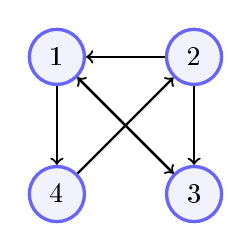
\begin{tikzpicture}[
		roundnode/.style={circle, draw=blue!60, fill=blue!5, very thick, minimum size=7mm},
		]
		%Nodes
		\node[roundnode]      (c1)                     {1};
		\node[roundnode]      (c2)       [right=of c1] {2};
		\node[roundnode]      (c3)       [below=of c2] {3};
		\node[roundnode]      (c4)       [below=of c1] {4};
		
		%Lines
		\draw[->,thick] (c1) -- (c3);
		\draw[->,thick] (c1) -- (c4);
		\draw[->,thick] (c2) -- (c3);
		\draw[->,thick] (c4) -- (c2);
		\draw[->,thick] (c3) -- (c1);
		\draw[->,thick] (c2) -- (c1);
		\end{tikzpicture}
	\end{center}
\end{minipage}
\begin{minipage}{0.5\textwidth}
	\begin{center}
		\[
		\begin{pmatrix}
		0 & 0 & \frac{1}{2} & \frac{1}{2} \\  
		\frac{1}{2} & 0 & \frac{1}{2} & 0 \\
		1 & 0 & 0 & 0 \\
		0 & 1 & 0 & 0 \\
		\end{pmatrix}
		\]
	\end{center}
\end{minipage}

\bigskip
\centerline{Példa: egy 4 oldalból álló web és linkmátrixa}
\bigskip

\subsection{Webekhez rendelt Markov-láncok}\label{markov_lancok}

Vegyünk egy lógó oldalt nem tartalmazó webet. Legyen adott egy úgynevezett véletlen szörföző, aki minden lépésben egyenletes eloszlás szerint választ a jelenlegi oldalon lévő linkek közül és továbbhalad a választott link által mutatott oldalra. A kezdeti eloszlás szintén legyen egyenletes.

Ehhez a modellhez rendelhetünk egy Markov-láncot, melynek állapotai a $V$ oldalhalmaz elemei, az átmenetvalószínűségeket pedig a linkmátrix adja meg:
 \[ p_{i,j} = (a_{i,j}) \quad i,j = 1,\ldots,|V| \text{,} \]
ahol $a_{i,j}$ az $A$ linkmátrix $i$. sorának $j$. eleme.

A Markov-lánchoz tartozó átmenetmátrix tehát éppen a linkmátrix lesz. A következő fejezetben igazoljuk, hogy a keresett PageRank vektor megoldása az $\bx = \bx A$ lineáris egyenletrendszernek. Látszik, hogy ez éppen a Markov-lánc invariáns eloszlása.

Ez logikus, hiszen az invariáns eloszlás mutatja, hogy hosszú távon az idő mekkora részét tölti a véletlen szörföző az állapotokban, tehát azok az oldalak lesznek a legfontosabbak, ahol várhatóan a legtöbb időt töltjük.

\vspace{0.1cm}
\textbf{Megjegyzés:} Nem minden webhez rendeletünk egy ilyen Markov-láncot. A lógó oldalakat tartalmazó webek linkmátrixában vannak csupa nulla sorok, melyek elrontják a mátrix sztochasztikusságát, de a \ref{link_web_logooldal} alfejezetben megadott helyettesítéssel kapott webek már megfelelőek. 
\vspace{0.1cm}

A linkmátrix 1 sajátértékének multiplicitása és a webhez rendelt Markov-lánc között kapcsolat van. Itt kimondunk egy tételt \cite{irreducible_closed}, amelynek segítségével meghatározhatjuk az 1 sajátérték multiplicitását a linkmátrix (mint átmenetmátrix) bizonyos tulajdonságaiból. Ez a későbbiekben (\ref{alfa_sajatertek}. fejezet) hasznos lesz. 

\begin{definicio}{Zárt részhalmaz}
	Egy átmenetmátrix elemeinek $H \subseteq V$ kommunikációs osztálya zárt, ha minden $i \in H$ és $j \notin H$ állapotok esetén a $p_{i,j}$ átmenetvalószínűség nulla.  
\end{definicio}

\begin{definicio}{Irreducibilis zárt részhalmaz}
	Egy átmenetmátrix elemeinek $H \in V$ részhalmaza irreducibilis zárt, hogyha zárt és egyetlen valódi részhalmaza sem zárt.
\end{definicio}

\begin{tetel}
	Egy átmenetmátrix esetén az 1 sajátérték multiplicitása megegyezik a mátrixban lévő irreducibilis zárt részhalmazok számával.
\end{tetel}

\section{A sajátértékprobléma}

Kapcsolat van az oldalak PageRankjának definíciójából kapott egyenletrendszer és a linkmátrix között. Ennek segítségével a PageRank definíciójából kapott egyenletrendszer felírható a következő mátrixegyenletként:
\[ 
\bx = \bx A, 
\]
%%% KP
ahol $\bx$ az oldalak rangjait tartalmazó sorvektor. Ezt átalakítva a következőt kapjuk:
\[
\bx^T = A^T \bx^T. 
\]
%%% KP
Ebből mátrixegyenletből látszik, hogy a keresett vektor az $A^T$ mátrix 1 sajátértékéhez 
tartozó sajátvektor. Mivel egy sajátvektor bármilyen nem nulla skalárszorosa is 
sajátvektor ezért az egyértelműség kedvéért tegyük fel, hogy az általunk keresett vektor 
az, ahol a komponensek összege 1. Ez azért hasznos, mert az előző fejezetben kiderült, 
hogy a PageRank vektor invariáns eloszlás is, ahol a komponensek összege éppen 1.

\vspace{0.1cm}
\textbf{Megjegyzés:} Ha webnek az internet egy sok oldalból álló részhalmazát választjuk (márpedig a PageRankokat ilyen esetre akarjuk kiszámolni), akkor a linkmátrix nagyon ritka lesz, azaz szinte az összes eleme 0. Ennek oka, hogy az egy oldal által linkelt további oldalak száma elenyésző az összes oldal számához képest. A linkmátrix ritkasága egy számolási szempontból nagyon kedvező tulajdonság. 

\subsection{Az 1 sajátérték}\label{egy_sajatertek}

Felmerül a kérdés, hogy minden $A^T$ mátrixnak sajátértéke-e az 1. Ehhez elég belátni, hogy az $A$ linkmátrixnak az 1 mindig sajátértéke, mivel egy mátrixnak és transzponáltjának a sajátértékei megegyeznek.

\begin{tetel}
	Az 1 sajátértéke minden lógó oldalt nem tartalmazó web linkmátrixának.
\end{tetel}
\begin{proof}
	Legyen $A$ egy tetszőleges, lógó oldalt nem tartalmazó, $n$ oldalból álló web linkmátrixa. Ekkor az $i$. sorhoz $(i = 1,2,\ldots,n)$ tartozó sorösszeg $ |v_i| \frac{1}{|v_i|} = 1 $, azaz minden ilyen mátrix sztochasztikus.
	
	Legyen $\be$ az $n$ komponensű oszlopvektor, melynek minden komponense 1. Ekkor az
	\[ A \be = \be \] 
	egyenlet teljesül, mert az eredményvektor $i$. komponense $(i = 1,2,\ldots,n)$
	\[ \sum_{j=1}^{n}{1 a_{i,j} } = 1, \] 
	a mátrix sztochasztikus tulajdonsága miatt. Tehát bármely linkmátrixnak az $\be$ vektor sajátvektora, 1 sajátértékkel.
\end{proof}
\vspace{0.5cm}

Ugyan bármely mátrixnak és transzponáltjának sajátértékei megegyeznek, de az nem igaz, hogy ezen sajátértékekhez tartozó sajátvektorok is azonosak, ezért a fenti tételben bevezetett $\be$ vektor nem biztos, hogy megoldása lesz a PageRank definíciója által meghatározott egyenletrendszernek. Ezzel a megoldás egyébként is használhatatlan az oldalak rangsorolásában, mivel minden oldalnak azonos rangot ad.

A lógó oldalakat tartalmazó webek esetén az 1 nem lesz mindig sajátértéke az $A^T$ mátrixnak (vannak 0 összegű sorok, amik a fenti bizonyítást elrontják), azonban figyeljük meg, hogy ha elvégezzük a \ref{link_web_logooldal} alfejezetben megadott helyettesítést akkor a kapott mátrix már sztochasztikus lesz, és erre már érvényes az előbbi tétel.

Tehát beláttuk, hogy minden ilyen mátrixnak vagy sajátértéke az 1, vagy egy egyszerű helyettesítéssel el lehet érni, hogy az legyen. 

\subsection{A legnagyobb sajátérték}\label{legnagyobb_sajatertek}

\begin{tetel}
	Minden lógó oldalt nem tartalmazó linkmátrix bármely $\lambda$ sajátértékre $ |\lambda| \leq 1$.
\end{tetel}
\begin{proof}
	A sajátértékek abszolút értékének felülről becsléséhez alkalmazzuk a Gershgorin körtételt. Eszerint a mátrix összes sajátértékének benne kell lennie legalább egy Gershgorin körben. A Gershgorin körtétel ugyan komplex mátrixokra is érvényes, de a linkmátrix csak valós elemeket tartalmazhat. A köröket meghatározó halmazok: 
	
	\[ K_i = \{ r \in \mathbb{R}: |r - a_{i,i}| \leq R_i \} \quad i = 1,2,\ldots,n \text{,} \]
	ahol $R_i$ az $i$. sorösszeg és $a_{i,i}$ az $i$. sorban lévő főátlóbeli elem.
	
	Már korábban beláttuk, hogy a feltételeknek eleget tévő linkmátrixok sztochasztikusak, azaz a sorösszeg minden sornál egy. A linkhalmaz \ref{link_web_logooldal} alfejezetben szereplő definíciójában nem engedjük meg azt, hogy egy oldal önmagára linkeljen, ezért $a_{i,i}$ minden sorra 0.
	
	Ezen állítások miatt a köröket meghatározó halmazok a következőre egyszerűsödnek minden sor esetén:
	
	\[ K_i = \{ r \in \mathbb{R}: |r| \leq 1 \} \quad i = 1,2,\ldots,n \]
	Ebből következik, hogy bármely $\lambda$ sajátértékre $ |\lambda| \leq 1$-nek teljesülnie kell.
\end{proof}

Beláttuk, hogy az egy minden esetben sajátérték, és azt is hogy ennél (abszolút értékben) nem is lehet nagyobb sajátérték. Ebből azonban nem következik az, hogy domináns is lenne. Előfordulhat olyan eset is, hogy a -1 is sajátérték, vagy az 1 többszörös multiplicitással szerepel.

\subsection{A hatványiteráció}

Ha sok oldalból álló webek esetén akarjuk meghatározni a rangokat, akkor a pontos megoldást adó módszerek nagyon lassúak, ezért közelítő, iteratív módszerre van szükség. Ideális választás a hatványiteráció alkalmazása az $A^T$ mátrixra, mert ebben az esetben elég tárolni mindössze a linkmátrix transzponáltját, és a PageRank vektor éppen aktuális iterációját a számoláshoz. A hatványiteráció általános alakja
\[ x^{i+1} = M x^i, \]
ahol $M \in \mathbb{R}^{n \times n}$ és $x^0 \in \mathbb{R}^n$.
\vspace{0.2cm}

A hatványiteráció azonban a domináns sajátértékhez tartozó sajátvektorhoz konvergál. Ha ilyen nincsen, akkor nem tudjuk garantálni a konvergenciát. Ahhoz, hogy alkalmazhassuk az egyhez tartozó sajátvektor megtalálására, vagy be kell látni, hogy az 1 mindig domináns sajátérték, vagy úgy kell módosítani a linkmátrixon, hogy az legyen.

\section{Konvergencia a PageRank vektorhoz}

\subsection{Gondot okozó tényezők}

Amikor egy nagy webhez tartozó PageRank vektort szeretnénk közelíteni, fontos tudni, hogy az iteráció úgy fog viselkedni ahogyan várjuk. A következő lehetőségeket kell ellenőrizni:

\begin{enumerate}
	\item Biztosan konvergálni fog-e a hatványiteráció?
	\item Ha igen, akkor az indítási helytől függetlenül mindig ugyanabba a vektorba? 
\end{enumerate}

Egyértelmű, hogy az indulási helytől független, biztos konvergenciát a \ref{legnagyobb_sajatertek} alfejezet végén említett szélsőséges esetek ronthatják el \cite{kleinproject}.

Ezek az eseten olyan webek esetén fordulnak elő, amelyek valójában több egymástól független (azaz nincsenek közöttük linkek) webből állnak össze \cite{kurt}.

\vspace{0.3cm}
\begin{minipage}{0.4\textwidth}
	\begin{center}
		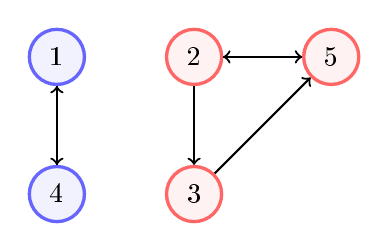
\begin{tikzpicture}[
				broundnode/.style={circle, draw=blue!60, fill=blue!5, very thick, minimum size=7mm},
			rroundnode/.style={circle, draw=red!60, fill=red!5, very thick, minimum size=7mm},
			]
			%Nodes
			\node[broundnode]      (c1)                     {1};
			\node[rroundnode]      (c2)       [right=of c1] {2};
			\node[rroundnode]      (c3)       [below=of c2] {3};
			\node[broundnode]      (c4)       [below=of c1] {4};
			\node[rroundnode]      (c5)       [right=of c2] {5};
			
			%Lines
			\draw[->,thick] (c1) -- (c4);
			\draw[->,thick] (c4) -- (c1);
			\draw[->,thick] (c2) -- (c3);
			\draw[->,thick] (c2) -- (c5);
			\draw[->,thick] (c3) -- (c5);
			\draw[->,thick] (c5) -- (c2);
		\end{tikzpicture}
	\end{center}
\end{minipage}
\begin{minipage}{0.5\textwidth}
	\begin{center}
		\[
		\begin{pmatrix}
		0 & 0 & 0 & 1 & 0 \\
		0 & 0 & \frac{1}{2} & 0 & \frac{1}{2} \\
		0 & 0 & 0 & 0 & 1 \\
		1 & 0 & 0 & 0 & 0 \\
		0 & 1 & 0 & 0 & 0 \\
		\end{pmatrix}
		\]
	\end{center}
\end{minipage}
\vspace{0.3cm}
\newline
\centerline{Két egymással nem érintkező "szubwebből" álló web és linkmátrixa.}
\vspace{0.3cm}

A fenti ábrán látható web linkmátrixának sajátértékei között szerepel a -1 és az 1 is, kétszeres multiplicitással.

\subsection{A konvergencia garantálása}\label{konvergencia_garantalas}

A domináns sajátérték (és ezzel együtt a konvergencia) létezésének garantálásához használjuk fel a \textbf{Perron–Frobenius tételt}:

\begin{tetel} Ha egy $A = (a_{i,j}) \in \mathbb{R}^{n \times n}$ mátrix minden eleme pozitív, akkor biztosan létezik domináns sajátérték, azaz ha a sajátértékek $\lambda_1 , \lambda_2 ,\ldots, \lambda_n$, akkor
\[ \exists r \in \{1,2,\ldots,n\}: \quad \forall i \neq r \quad |\lambda_i| < \lambda_r.  \]
\end{tetel}

A tétel értelmében tehát az egyértelmű PageRank vektor létezéséhez annyit kell tenni, hogy a linkmátrixot úgy módosítjuk, hogy csak pozitív elemei legyenek.

\begin{definicio}{Google mátrix}
	Legyen $A \in \mathbb{R}^{n \times n}$ egy lógó oldalt nem tartalmazó web linkmátrixa, $S$ pedig egy egy olyan $n \times n$-es mátrix, melynek minden eleme $\frac{1}{n}$. Ekkor a Google mátrix definíció szerint
	\[ G := \alpha A + (1-\alpha) S, \qquad \alpha \in [0,1] \]
\end{definicio}
\vspace{-1cm}

Látható, hogy a Google mátrix értéke függ az $\alpha$ paramétertől, de majdnem minden esetben (az $\alpha = 1$-et kivéve) a kapott mátrix minden eleme biztosan pozitív, azaz létezik domináns sajátérték és a hatványiteráció indulási helytől függetlenül az ehhez tartozó sajátvektorhoz fog konvergálni.

\[A =
\begin{pmatrix}
0 & \frac{1}{2} & \frac{1}{2} & 0 \\
\frac{1}{3} & 0 & \frac{1}{3} & \frac{1}{3} \\
\frac{1}{3} & \frac{1}{3} & 0 & \frac{1}{3} \\
0 & 0 & 1 & 0 \\
\end{pmatrix},
S =
\begin{pmatrix}
\frac{1}{4} & \frac{1}{4} & \frac{1}{4} & \frac{1}{4} \\
\frac{1}{4} & \frac{1}{4} & \frac{1}{4} & \frac{1}{4} \\
\frac{1}{4} & \frac{1}{4} & \frac{1}{4} & \frac{1}{4} \\
\frac{1}{4} & \frac{1}{4} & \frac{1}{4} & \frac{1}{4} \\
\end{pmatrix},
G =
\begin{pmatrix}
0,\!038 & 0,\!463 & 0,\!463 & 0,\!038 \\
0,\!321 & 0,\!038 & 0,\!321 & 0,\!321 \\
0,\!321 & 0,\!321 & 0,\!38 & 0,\!321 \\
0,\!038 & 0,\!038 & 0,\!888 & 0,\!038 \\
\end{pmatrix}
\]

\vspace{0.1 cm}
\centerline{Egy web linkmátrixa, az $S$ mátrix és az $\alpha = 0,7$ paraméterrel kapott Google mátrix.}

\subsection{A Google mátrixhoz rendelt Markov-lánc}\label{google_matrix_markov}

A linkmátrixhoz hasonlóan a Google mátrixhoz is rendelhető egy Markov-lánc ez is sztochasztikus mátrix (ennek rövid igazolása a következő fejezet elején található). Az ehhez a mátrixhoz tartozó Markov-lánc néhány tulajdonságát a következő tétel mondja ki.

\begin{tetel}
	A Google mátrixhoz tartozó Markov-lánc irreducibilis és aperiodikus.
\end{tetel}
\begin{proof}
	Mindkét tulajdonság következik abból, hogy a Google mátrixot úgy konstruáltuk, hogy egy elem se lehessen benne nulla. Az irreducibilitás azt jelenti, hogy bármely állapotból bármely másikba el lehessen jutni, és az, hogy nincs nulla az átmenetmátrixban éppen ezt jelenti. 
	
	Az aperiodikusságot az garantálja, hogy a fentiek miatt a főátlóbeli elemek sem nullák, ezért a Markov-láncnak nem lehet semmilyen egytől különböző periódusa.
\end{proof}

\noindent
\textbf{Megjegyzés:} \textit{(A helyettesítés mögötti heurisztika.)} \newline
Tekintsük a webhez rendelt Markov-láncot. Ezt úgy módosítjuk, hogy a véletlen szörföző most már nem csak a linkeken keresztül juthat el a következő oldalra, hanem $1-\alpha$ valószínűséggel egy egyenletes eloszlás szerint választott véletlen oldalra ugrik. Ebben a modellben már nem lehetnek teljesen különálló oldalhalmazok, a véletlen szörföző bárhonnan eljuthat bárhova.

Az így kapott Markov-lánc átmenetmátrixa éppen a Google mátrix lesz, ahol az $\alpha$ paraméter dönt arról, hogy mekkora valószínűséggel követjük a linkeket és mekkorával ugrunk véletlen oldalra.

\section{A Google mátrix és az $\alpha$ paraméter}

\subsection{A Google mátrix tulajdonságai}\label{google_matrix_tul}

A Google mátrix szintén sztochasztikus lesz, bármely $\alpha$ paraméter esetén. A linkmátrixról ($A$) és a csupa $1/n$ komponensből álló ($S$) mátrixokról tudjuk, hogy sztochasztikusak, ezért $\alpha A$ és $(1-\alpha)S$ mátrixok sorösszegei rendre $\alpha$ és $(1-\alpha)$. A Google mátrix esetén így a sorok összege $\alpha+(1-\alpha) = 1$ lesz.

A hatványiterációt nem a Google mátrixra, hanem a transzponáltjára kell alkalmaznunk, ami a linkmátrix és az $S$ mátrix segítségével a 

\[ G^T = (\alpha A + (1-\alpha)S)^T = \alpha A^T + (1-\alpha) S^T \]
alakban írható fel.

\vspace{0.2cm}

A \ref{linkmatrix} alfejezetben említettük, hogy a linkmátrix általában egy ritka mátrix és hogy ez számítási szempontból nagyon előnyös. A Google mátrix ennek éppen az ellentéte, nemhogy sűrű, de biztosan nem tartalmaz egyetlen 0 elemet sem, ugyanis ez szükséges ha a hatványiteráció konvergenciáját a Perron–Frobenius tétellel akarjuk garantálni. Sűrű mátrixok esetében azonban a mátrixszorzás sokkal lassabb mint ritkáknál.

A Google mátrix sűrűségéből adódó számítási problémát ki lehet küszöbölni. Ha hatványiteráció $i$.-ik lépése

\[ \bx^{i+1} = G^T \bx^i, \]
ahol $\bx$ a PageRank oszlopvektor, akkor ez ekvivalens a következő alakkal:

\[ \bx^{i+1} = \alpha A^T \bx^i + \frac{(1-\alpha)}{n} \bx^i. \] 

Először tehát $A^T$ skalár szorosával szorozzuk a PageRank vektor jelenlegi iterációját, majd ezután adjuk hozzá a csupa $\frac{1-\alpha}{n}$ elemekből álló vektort. Ekkor az elvégzett mátrixszorzásban már nem szerepel a sűrű Google mátrix, de az iteráció eredménye ugyanaz, mintha azzal szoroztunk volna. 

\subsection{Az $\alpha$ paraméter kérdése}

Az előző fejezetben láttuk, hogy szinte bármilyen $\alpha \in [0,1]$ választás esetén (az $\alpha=1$ esetet kivéve) garantáljuk a hatványiteráció konvergenciáját, de felmerül a kérdés, hogy van-e egyéb jelentősége ennek a paraméternek, és ha igen, akkor hogyan válasszuk meg.

A \ref{google_matrix_markov} alfejezetben megadott heurisztikából kiderül, hogy $\alpha$ nem lesz más, mint annak a valószínűsége, hogy a véletlen szörföző követi a linkeket, ahelyett, hogy tetszőleges oldalra ugrana. Mivel az oldalak fontosságát a linkek alapján szeretnénk meghatározni (és a PageRankot is így definiáltuk), ezért adódik, hogy $\alpha$-t válasszuk az egyhez minél közelebbi értéknek, mert így a web struktúrája, a linkek nagy hangsúlyt kapnak a Google mátrixban is. Az egyhez közeli $\alpha$ azt jelenti, hogy a véletlen szörföző szinte mindig a linkeken keresztül halad tovább.

Tudjuk azonban, hogy a Google, saját PageRank számolásánál $\alpha \approx 0,85$ \cite{lang2} értéket használ. A fentiek ismeretében miért nem 0,9 vagy akár 0,999 ez az érték? 

A válasz az, hogy $\alpha$-tól nagyban függ a konvergencia sebessége, amit a következő fejezetekben indoklunk.

\subsection{A hatványiteráció konvergenciájának sebessége}\label{konvergencia_sebesseg}

Legyenek a mátrixnak, melyre a hatványiterációt szeretnénk alkalmazni a következők a sajátértékei:

\[ |\lambda_1| > |\lambda_2| \geq |\lambda_3| \geq \ldots \geq |\lambda_n|. \] 

Látható, hogy $\lambda_1$ domináns sajátérték, azaz a hatványiteráció biztosan konvergálni fog. A valódi sajátvektor és az iteráció eredménye közti különbség minden lépésben aszimptotikusan csökken $ |\lambda_1| / |\lambda_2|$ valamilyen többszörösével \cite{poweriteration}.

$\lambda_1$ domináns sajátérték, ezért a vizsgált hányadosról biztosan tudjuk, hogy
\[ 1 < |\lambda_1| / |\lambda_2|. \]

Látható, hogy minél kisebb ez a hányados, annál kisebb mértékben fog csökkenni a hiba mértéke az iterációs lépések között, azaz a konvergencia sebessége akkor a legrosszabb amikor $|\lambda_1| / |\lambda_2| \approx 1$, azaz $|\lambda_1| \approx |\lambda_2|$. A Google mátrix estében a sajátértékek:
\[ 1 > |\lambda_2| \geq |\lambda_3| \geq \ldots \geq |\lambda_n|, \]
ezért a fentebb említett legrosszabb eset a következőképpen módosul:
\[ 1 / |\lambda_2| \approx 1. \]

Minél közelebb van tehát a második legnagyobb sajátérték egyhez (a domináns sajátértékhez), annál lassabb lesz a konvergencia sebessége. A Google mátrixra alkalmazott hatványiteráció konvergenciájának pontos sebességét a \ref{alfa_sajatertek} alfejezet végén adjuk meg, mivel ehhez a következő alfejezetben bizonyított ismeretek kellenek.

\subsection{$\alpha$ mint sajátérték}\label{alfa_sajatertek}

A konvergencia sebessége úgy kapcsolódik az $\alpha$ paraméterhez, hogy $\alpha$ maga is sajátérték (a legtöbb esetben). Ezt az alábbi két tétel igazolja \cite{secondeigenvalue}. 

\vspace{0.1cm}
\begin{tetel}
		Ha a Google mátrix $G = \alpha A + (1-\alpha)S$ ($\alpha \in [0,1)$, $G \in \mathbb{R}^{n \times n}$) sajátértékei $ 1 > |\lambda_2| \geq |\lambda_3| \geq \ldots \geq |\lambda_n|$, akkor $\lambda_2 \leq \alpha$.
\end{tetel}
\begin{proof}
	
	Először igazoljuk a tételt az $\alpha = 0$ esetre. Ekkor $G = S$, ahol $S = (\frac{1}{n})_{i,j}$ $(i,j = 1,2,\ldots,n)$.
	Ekkor $S = \be \be_p^T$, ahol $\be$ a csupa egyeseket, $\be_p$ pedig a csupa $\frac{1}{n}$ komponenseket tartalmazó oszlopvektorok. Mivel $S$ felírható ilyen alakban, ezért $Rank(S) = 1$, ami miatt csak két sajátérték lehetséges: 1, mivel ($\be^T \be_p = 1$) és 0 \cite{rankonematrix}. A második legnagyobb sajátérték tehát 0 és az egyenlőtlenség teljesül.
	
	\vspace{0.1cm}
	\noindent
	Az általános $0 < \alpha < 1$ esetet a következő lemmák segítségével igazoljuk. 
	
	\begin{lemma}\label{orthogonal_lemma}
	 	A $G^T$ mátrix $\lambda_2$ sajátértékhez tartozó sajátvektor (legyen $\bx_2$) ortogonális az $\be$ vektorra, vagyis $\be^T \bx_2 = 0$.
	\end{lemma}
	\begin{proof}
		Tudjuk, hogy egy mátrixhoz és transzponáltjához tartozó sajátvektorok ortogonálisak, ha nem ugyanahhoz a sajátértékhez tartoznak \cite{orthogonal_eigenvectors}. Mivel $\bx_2$ a $\lambda_2$-höz tartozik $G^T$ mátrixban, ezért ortogonális lesz $G$ legnagyobb sajátértékéhez tartozó sajátvektorra. 
		
		Ez a sajátvektor éppen $\be$, mivel $ G \be = \be$, amiből
		\[  ( \alpha A + (1-\alpha) S ) \be = \be  \]
		\[  \alpha A \be + (1-\alpha) S \be = \be \]
		A \ref{egy_sajatertek} fejezetben láttuk, hogy $A \be = \be$ és az is igaz, hogy $S \be = \be$, ezért az egyenlőség teljesül, $\be$ valóban sajátvektora $G$-nek, és ortogonális $\bx_2$-re.	
	\end{proof}
	
	\begin{lemma}
		Legyen $\bx_2$ a $\lambda_2$ sajátértékhez tartozó sajátvektor a $G^T$ mátrixban. Ekkor $S^T \bx_2 = 0$.
	\end{lemma}
	\begin{proof}
		Tudjuk, hogy $S = \be \be_p^T$, vagyis $S^T = \be_p \be^T$. Ekkor $S^T \bx_2 = \be_p \be^T \bx_2$. Az előző lemmából tudjuk, hogy $\be^T \bx_2 = 0$, ezért $S \bx_2$ is 0 lesz.
	\end{proof}
	
	\begin{lemma}
		$\bx_2$ vektor sajátvektora lesz $A$-nak is, és ha a hozzá tartozó sajátérték $\mu$, akkor $\mu = \lambda_2 / \alpha$. 
	\end{lemma}
    \begin{proof}
    	Az $\bx_2$ vektor a $G^T$ mátrix $\lambda_2$ sajátértékéhez tartozó sajátvektor, azaz $G^T \bx_2 = \lambda_2 \bx_2$. Ha behelyettesítünk a $G = \alpha A + (1-\alpha)S$ helyettesítéssel, akkor
    	\[ (\alpha A^T + (1-\alpha) S^T ) \bx_2 = \lambda_2 \bx_2. \]
    	Az előző lemmából tudjuk, hogy $S^T \bx_2 = 0$, ezért 
    	\[ \alpha A^T \bx_2 = \lambda_2 \bx_2. \]
    	Mivel az $\alpha = 0$ esetet külön bizonyítottuk, feltehetjük, hogy $\alpha \neq 0$ és oszthatunk vele, amiből
    	\[ A^T \bx_2 = \frac{\lambda_2}{\alpha} \bx_2 \]
    	adódik. Legyen $\lambda_2/\alpha = \mu$, ekkor
    	\[ A^T \bx_2 = \mu \bx_2. \]

    	Látható, hogy $\bx_2$ valóban sajátvektora $A^T$-nek is, és a hozzátartozó sajátérték éppen $\mu = \lambda_2/\alpha$.
    \end{proof}
	
	Az előző lemmából tudjuk, hogy $\lambda_2 = \mu \alpha$, továbbá $A$, a linkmátrix sztochasztikus, ezért $|\mu| \leq 1$. Ezekből következik, hogy $ |\lambda_2| < \alpha $ (mivel egynél kisebb számmal kellett szorozni, hogy egyenlőek legyenek).
\end{proof}

A bizonyítás során azért nem foglalkoztunk az $\alpha = 1$ esettel, mert ekkor a Google mátrix a linkmátrix lesz, és még a konvergenciát sem tudjuk garantálni.

\begin{tetel}
	Ha a Google mátrix $G = \alpha A + (1-\alpha)S$ ($\alpha \in [0,1)$, $G \in \mathbb{R}^{n \times n}$) sajátértékei $ 1 > |\lambda_2| \geq |\lambda_3| \geq \ldots \geq |\lambda_n |$ és $A$-ban van legalább kettő irreducibilis zárt részhalmaz, akkor $\lambda_2 = \alpha$.
\end{tetel}
\begin{proof}
	Az $\alpha = 0$ esetre a tételt már az előző bizonyítás elején beláttuk. A $0 < \alpha < 1$ esetet a következő két lemma segítségével igazoljuk.
	
	\vspace{0.1cm}
	\textbf{Jelölések:} Legyen $\by_i$ az $A^T$ transzponált linkmátrix $i$. sajátvektora, $\mu_i$ pedig az ehhez tartozó sajátérték. Legyen $\bx_i$ a $G^T$ transzponált Google mátrix $i$. sajátvektora. Az előző bizonyításhoz hasonlóan $S = \be \be_p^T$, ahol $\be$ a csupa egyeseket, $\be_p$ pedig a csupa $\frac{1}{n}$ komponenseket tartalmazó oszlopvektorok.
	
	\begin{lemma}
		$A^T$ bármely $\by_i$ sajátvektora, amelyik ortogonális az $\be$ vektorra, a $G^T$ mátrixnak is sajátvektora lesz. Továbbá ekkor $\lambda_i = \alpha \mu_i$.
	\end{lemma}
	\vspace{-0.5cm}
	\begin{proof}
		Tudjuk, hogy $\be^T \by_i = 0$, ezért
		\[ S^T \by_i = (\be \be_p^T)^T \by_i = \be_p \be^T \by_i = 0. \]
		Ha kiírjuk a $G^T \by_i$ szorzatot, akkor
		\[ (\alpha A^T + (1-\alpha) S^T ) \by_i = \alpha A^T \by_i + (1-\alpha) S^T \by_i = \alpha A^T \by_i \]
		adódik. A sajátérték definíciója alapján $A^T \by_i = \mu_i \by_i$, ezért a fenti kifejezés megegyezik $\alpha \mu_i \by_i$-vel. Tehát
		\[ G^T \by_i = (\alpha \mu_i) \by_i, \]
		vagyis $\by_i$ valóban sajátvektora lesz $G^T$-nek a $\alpha \mu_i$ sajátértékkel.
	\end{proof} 

	\begin{lemma}
		$\exists i \in \{ 1,2,\ldots,n \}$, hogy $\lambda_i = \alpha$.
	\end{lemma}
	\vspace{-0.5cm}
	\begin{proof}
		Keressük az $\bx$ vektort, mely sajátvektora $P$-nek és ortogonális az $\be$ vektorra. A \ref{markov_lancok}. fejezetben lévő tétel alapján az 1 sajátérték multiplicitása legalább kettő, mivel legalább ennyi irreducibilis zárt részhalmaz van $A^T$ mátrixban. Ekkor biztosan létezik két lineárisan független sajátvektor, melyek az egy sajátértékhez tartoznak, legyenek ezek $\by_1,\by_2$. Ekkor
		
		\[ k_1 = \by_1^T \be, \]
		\[ k_2 = \by_2^T \be. \]
		Definiáljuk a keresett $\bx$ vektort a következőképpen:
		\begin{equation*}
		\bx=\begin{cases}
		\frac{\by_1}{k_1} - \frac{\by_2}{k_2}, & \text{ha $k_1,k_2 \neq 0$},\\
		\by_1, & \text{ha $k_1 = 0$}, \\
		\by_2, & \text{ha $k_2 = 0$}. 
		\end{cases}
		\end{equation*}
		\noindent
		Ekkor $\bx$ sajátvektora $A^T$-nek, az 1 sajátértékhez tartozik és ortogonális $\be$-re. A második és harmadik esetben ez egyértelműen látszik, az első esetben azért igaz, mert 
		\[ A^T (\frac{\by_1}{k_1} - \frac{\by_2}{k_2}) = \frac{\by_1}{k_1} - \frac{\by_2}{k_2} \] 
		\[ \frac{A^T \by_1}{k_1} - \frac{A^T \by_2}{k_2} = \frac{\by_1}{k_1} - \frac{\by_2}{k_2}, \]
		és $\by_1,\by_2$-ről tudjuk, hogy sajátvektorai $A^T$-nek az 1 sajátértékkel ezért $A^T \by_1 = \by_1$, $A^T \by_2 = \by_2$ és az egyenlőség teljesül. 
		
		Az előző lemma miatt ekkor $\bx$ $G^T$-nek is sajátvektora lesz, méghozzá az $\alpha$ sajátértékkel.  
	\end{proof} 

	Ekkor tehát $G^T$-nek biztosan sajtértéke $\alpha$ és $\lambda_2 \geq \alpha$, mivel $\lambda_2$ a második legnagyobb sajátérték, $\alpha$ pedig biztosan nem lehet a legnagyobb, mert az egy. Az előző tétel viszont garantálja, hogy $\lambda_2 \leq \alpha$. A két egyenlőtlenség csak akkor teljesülhet egyszerre, ha $\lambda_2 = \alpha$.
\end{proof}
\vspace{0.2cm}

A tétel feltétele, vagyis az, hogy a linkmátrixban van legalább kettő irreducibilis zárt részhalmaz ugyan nem teljesül minden web linkmátrixára, de a sok oldalból álló webek estén szinte bisztosan igaz lesz, a linkmátrix \ref{linkmatrix}. fejezet megjegyzésében említett ritkasága miatt.

Láttuk tehát, hogy $\alpha$ a vizsgált mátrix második legnagyobb sajátértéke, ezért az \ref{konvergencia_sebesseg} alfejezet értelmében a hatványiteráció konvergenciájának sebessége függ $\alpha$-tól. Ezt a sebességet a következő tétel adja meg pontosan \cite{convergence_speed}:

\begin{tetel}
	Legyen $\mathbf{\pi}$ a PageRank vektor, $\bx^i$ pedig a Google mátrixra alkalmazott hatványiteráció $i$. lépésének erdeménye. Ekkor $\exists C \in \mathbb{R}$:
	\[ \Vert \bx^i - \mathbf{\pi} \Vert \leq C \alpha^i, \quad i = 1,2,\ldots \]
\end{tetel}

\textbf{Megjegyzés:} Ha a második tétel feltétele nem is teljesül, az első tétel akkor is érvényes. Ez azt jelenti, hogy nem ismerjük ugyan pontosan a második legnagyobb sajátértéket (és ezzel együtt a konvergencia sebességét), de felülről tudjuk becsülni $\alpha$-val.

\section{Algoritmus a PageRank meghatározására}

Megadunk egy algoritmust a PageRank kiszámolására és a weboldalak fontosság szerinti sorba állítására, ami az előző fejezetekben leírtakon alapul. Az \ref{program} alfejezetben említett program is ezt a módszert használja.

\subsection{Algoritmus általános web esetén}

Legyen adott egy tetszőleges, $n$ oldalból álló web.

\begin{enumerate}[label=(\Roman*)]
	\item Adjuk meg a webhez tartozó $A = (a_{i,j})$ linkmátrixot, a \ref{linkmatrix} fejezetben megadott képlet alapján: 
	\begin{equation*}
	a_{i,j}=\begin{cases}
	\frac{1}{ |v_i| }, & \text{ha $(v_i,v_j) \in L$}.\\
	0, & \text{egyébként}.
	\end{cases}
	\end{equation*}
	A használt jelölések magyarázata a fent említett fejezetben található.
	
	\item Végezzük el a helyettesítést a lógó oldalak kiküszöbölésére, azaz ha az $n \times n$-es linkmátrixban van csupa nulla sor, azt cseréljük le $1/n$ elemekből álló sorra.
	
	\item Válasszunk egy $\alpha \in (0,1)$ paramétert, figyelembe véve azt, hogy a túl kicsi érték elnyomja a linkek szerkezetét, az egyhez túl közeli pedig nagyon lelassítja a hatványiteráció konvergenciáját. Konstruáljuk meg a Google mátrixot ezzel a paraméterrel:
	\[G = \alpha A + (1-\alpha)S,\]
	ahol $S$ egy csupa $1/n$ elemekből álló $n \times n$-es mátrix. 
	
	\item Végezzük a hatványiterációt a $G^T$ mátrixon, amíg a két iterációs lépés közötti különbség nem csökken valami kicsi $\epsilon$ érték alá, vagy adjunk meg konkrét iterációs lépésszámot. Az $x_0$ kiindulási pont legyen a csupa $1/n$ komponensekből álló vektor.
	
	\textbf{Megjegyzés:} Az iterációt ne közvetlenül a sűrű $G^T$ mátrixon, hanem az \ref{google_matrix_tul} alfejezetben említett
	\[ x^{i+1} = \alpha A^T x^i + (1-\alpha) S^T \] 
	felbontás szerint végezzük, mert így csak a ritka linkmátrixal kell szorozni.
	
	\item Az iteráció eredménye a PageRank vektor közelítése, ahol az $i.$ komponens az $i.$ oldal fontosságát adja meg. Rendezzük a komponenseket csökkenő sorrendbe, így kapjuk az oldalak fontossági rangsorát.
	
\end{enumerate}

\subsection{Példa}

Végrehajtjuk az előző alfejezetben leírt algoritmust egy konkrét webre, ez legyen a lenti ábrán látható irányított gráf.
\begin{figure}[h]
	\centering
	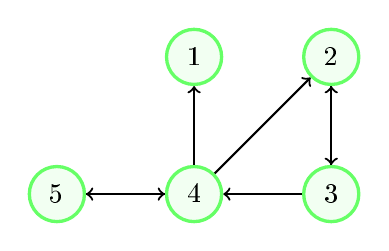
\begin{tikzpicture}[
	roundnode/.style={circle, draw=green!60, fill=green!5, very thick, minimum size=7mm},
	]
	\centering
	%Nodes
	\node[roundnode]      (c1)                     {1};
	\node[roundnode]      (c2)       [right=of c1] {2};
	\node[roundnode]      (c3)       [below=of c2] {3};
	\node[roundnode]      (c4)       [below=of c1] {4};
	\node[roundnode]      (c5)       [left=of c4] {5};
	
	%Lines
	\draw[->,thick] (c2) -- (c3);
	\draw[->,thick] (c3) -- (c2);
	\draw[->,thick] (c3) -- (c4);
	\draw[->,thick] (c4) -- (c1);
	\draw[->,thick] (c4) -- (c2);
	\draw[->,thick] (c4) -- (c5);
	\draw[->,thick] (c5) -- (c4);
	\end{tikzpicture}
\end{figure}

\begin{enumerate}[label=(\Roman*)]
\item A gráfról leolvasható linkmátrix a következő lesz:
\vspace{-1cm}
\begin{center}
	\[
	\begin{pmatrix}
	0 & 0 & 0 & 0 & 0 \\
	0 & 0 & 1 & 0 & 0 \\
	0 & \frac{1}{2} & 0 & \frac{1}{2} & 0 \\
	\frac{1}{3} & \frac{1}{3} & 0 & 0 & \frac{1}{3} \\
	0 & 0 & 0 & 1 & 0 \\
	\end{pmatrix}.
	\]
\end{center}

\item Látható, hogy az első oldal egy lógó oldal, ugyanis nincs belőle kimenő link, ezért a linkmátrixban helyettesítést kell alkalmaznunk az első sorban. A módosított linkmátrix ezért
\vspace{-1cm}
\begin{center}
	\[
	\begin{pmatrix}
	\frac{1}{5} & \frac{1}{5} & \frac{1}{5} & \frac{1}{5} & \frac{1}{5} \\
	0 & 0 & 1 & 0 & 0 \\
	0 & \frac{1}{2} & 0 & \frac{1}{2} & 0 \\
	\frac{1}{3} & \frac{1}{3} & 0 & 0 & \frac{1}{3} \\
	0 & 0 & 0 & 1 & 0 \\
	\end{pmatrix}.
	\]
\end{center}

\item Válasszuk az $\alpha = 0,85$ értéket, a konvergencia sebessége és a linkek szerkezete közötti kompromisszumként. A Google mátrixot a 
\vspace{-1cm}
\begin{center}
	\[0,85
	\begin{pmatrix}
	\frac{1}{5} & \frac{1}{5} & \frac{1}{5} & \frac{1}{5} & \frac{1}{5} \\
	0 & 0 & 1 & 0 & 0 \\
	0 & \frac{1}{2} & 0 & \frac{1}{2} & 0 \\
	\frac{1}{3} & \frac{1}{3} & 0 & 0 & \frac{1}{3} \\
	0 & 0 & 0 & 1 & 0 \\
	\end{pmatrix}
	+ 0,15 
	\begin{pmatrix}
	\frac{1}{5} & \frac{1}{5} & \frac{1}{5} & \frac{1}{5} & \frac{1}{5} \\
	\frac{1}{5} & \frac{1}{5} & \frac{1}{5} & \frac{1}{5} & \frac{1}{5} \\
	\frac{1}{5} & \frac{1}{5} & \frac{1}{5} & \frac{1}{5} & \frac{1}{5} \\
	\frac{1}{5} & \frac{1}{5} & \frac{1}{5} & \frac{1}{5} & \frac{1}{5} \\
	\frac{1}{5} & \frac{1}{5} & \frac{1}{5} & \frac{1}{5} & \frac{1}{5} \\
	\end{pmatrix}
	\]
\end{center}
egyenletből kapjuk:
\vspace{-1cm}
\begin{center}
	\[G =
	\begin{pmatrix}
	0,\!2 & 0,\!2 & 0,\!2 & 0,\!2 & 0,\!2 \\
	0,\!03 & 0,\!03 & 0,\!88 & 0,\!03 & 0,\!03 \\
	0,\!03 & 0,\!455 & 0,\!03 & 0,\!455 & 0,\!03 \\
	0,\!313 & 0,\!313 & 0,\!03 & 0,\!03 & 0,\!313 \\
	0,\!03 & 0,\!03 & 0,\!03 & 0,\!88 & 0,\!03 \\
	\end{pmatrix}
	\]
\end{center} 

\item Végezzük el a hatványiteráció első 5 lépését $G^T$ mátrixra. A kapott eredményvektorok sorvektor formában:
% KP a tizedesvesszo tul nagy helyet hagy, ezert kell a \! (kis negativ koz)
% eleg szoszmotolos
\[
\begin{split}
x_0 & = ( 0,\!2, \ \,0,\!2, \! \ \, 0,\!2 ,\ \, 0,\!2 ,\ \, 0,\!2   ) \\
x_1 & = (  0,\!121 ,\ \, 0,\!206 ,\ \, 0,\!234 ,\ \ 0,\!319 ,\ \, 0,\!121 )\\   
x_2 & = (  0,\!141 ,\ \, 0,\!24,\ \ 0,\!225 ,\ \, 0,\!253 ,\ \, 0,\!141 )\\   
x_3 & = (  0,\!126 ,\ \, 0,\!221 ,\ \, 0,\!258 ,\ \, 0,\!269 ,\ \, 0,\!126) \\  
x_4 & = (  0,\!128 ,\ \, 0,\!237 ,\ \, 0,\!239 ,\ \, 0,\!268 ,\ \, 0,\!128 )\\  
x_5 & = (  0,\!128 ,\ \, 0,\!229 ,\ \, 0,\!253 ,\ \, 0,\!262 ,\ \, 0,\!128 ). 
\end{split}
\]
Ilyen kis méretű mátrix esetén nem jelent nehézséget a valódi sajátérték vektor 
meghatározása. A PageRank vektor ebben az esetben
\[\begin{pmatrix} 0,128 & 0,235 & 0,252 & 0,268 & 0,128 \\ \end{pmatrix},\]
ami jól láthatóan közel van az iteráció eredményéhez, már az ötödik lépés után.

\item Rendezzük sorba és rendeljük hozzá az oldalakhoz a kapott fontossági pontszámokat. Az eredmény leolvasható a táblázatból.
\begin{center}
	\begin{tabular}{c | c}
		4. oldal & 0,268 \\
		\hline
		3. oldal & 0,252 \\
		2. oldal & 0,235 \\
		5. oldal & 0,128 \\
		1. oldal & 0,128 \\
	\end{tabular}
\end{center}
\end{enumerate}
A legfontosabb oldal tehát a negyedik. A rangsorolást nehezíti, hogy a első és az ötödik oldal pontszáma annyira közel van egymáshoz, hogy 3 tizedesjegy pontossággal nem is lehet őket megkülönböztetni.

%hivatkozások ---------------------------------------------------------
\bibliography{hivatkozasok}
\bibliographystyle{plain}

\end{document}